\chapter{Local Correlation: Excited State}

The previous chapter demonstrated how it is possible to achieve low to linear computational complexity for Hartree Fock as well as M{\o}ller-Plesset perturbation theory and Coupled Cluster. Highly optimized code has been developped for all of them, exploiting distributed memory parallelism and/or accelerators such as GPUs. The local treatment of electron correlation can naturally be extended to excited states as well. The development of low-scaling excited states has been steadily progressing since the early 2000s, and many competing flavors have emerged over the years both for the Algebraic Diagrammtic Construction method, Coupled Cluster linear response, and Equation-of-Motion Coupled Cluster. Local excited state methods need to take into considerations both local electron correlation, as well as the local character of the excited state itself.

% Bau2017 CornFlex https://aip.scitation.org/doi/pdf/10.1063/1.4984820

\section{Excited State Methods in the Atomic Orbital Basis}


\section{Low Scaling ADC, CCLR and EOM-CC using Molcular Orbitals}

Virtually all existing low-scaling implementations of ADC, CCLR and EOM-CCSD use some form of local or compact molecular orbital representation, to varying degrees of success. The major problem that these methods face is the non-locality of certain excited states such as charge transfer states (Figure ...), which can involve occupied and virtually orbitals which are localized on entirely different parts in the system. Clearly, truncating virtual orbitals spatially is no longer a valid option, and makes a straight-forward extension of LMO-methods difficult, becuase they cut out far-away contributions. Similarly, the excited state is often not properly described by the electronic ground state (pair-)densities and their associated (pair) natural representation. Over the years, various strategies have been proposed to adapt exisiting LMO, NO and PNO schemes to excited states as well. 

\subsection{Orbital Invariant ADC/CCLR/EOM-CCSD}

Similarly to ground state MP and CC methods, the working equations can be reformulated to work with any orbital representation. Consider for example the general ADC(2) working excitations for computing the singles and doubles vectors
\begin{equation}
\begin{split}
r_{ia} = A_{ia,jb} u_{jb} + A_{ia,jbkc} u_{jbkc} \\
r_{iajb} = A_{iajb,kc} u_{kc} + A_{iajb,kcdl} u_{kcdl}
\end{split}
\end{equation}
\noindent Transforming to the local basis is straight-forward: the trial vectors $u_{ia}$, as well as the molecular electron integrals $\cn{ia}{jb}$ and MP2 amplitudes $t_{iajb}$ in the Jacobian $\mathbf{A}$ (see Section ...) are simply replaced by their local counterparts $u_{\uli\ola}$, $\cn{\uli\ola}{\ulj\olb}$ and $t_{\uli\ola\ulj\olb}$. The local MP2 amplitudes are computed using either the Hylleraas functional (Equation ...) or the Laplace transform (Equation ...). Similar things apply for an orbital-invariant formulation of CCLR and EOM-CCSD. 

ADC(2) and CC2 variants also allow an on-the-fly computation of the doubles part (see ...). Here, the orbital invariant formaulation becomes less straight-forward becuase the doubles-doubles block of the ADC and CC2 Jacobian matrix is no longer diagonal, similar to the Fock matrix. Fortunately, the Laplace transform can be applied to circumvent this problem, in this case shown for ADC(2)
\begin{equation}
\begin{split}
r_{ia}(\omega) &= A_{ia,jb} u_{jb} + A_{ia,jbkc} \frac{A_{iajb,kc} u_{kc}}{\omega - \eps_a - \eps_b + \eps_i + \eps_j} \\
&= A_{ia,jb} u_{jb} - \sum_{\alpha}^{n} |w\pa| e^{\left(\omega - \eps_a - \eps_b + \eps_i + \eps_j\right) tpa} A_{ia,jbkc} A_{,kc} u_{kc} 
\end{split}
\end{equation}
Using a similar apporach to Equation ..., the local ADC(2) equations are then given by 
\begin{equation}
r_{\uli \ola}(\omega) = A_{\uli \ola, \ulj \olb} u_{\ulj \olb} - A_{\uli \ola, \ulj \olb \ulk \olc} \sum_{\alpha}^{n} e^{\omega t\pa} X_{\ulj \ulj'}\pa Y_{\olb \olb'}\pa A_{\ulj' \olb' \ulk' \olc', \ull \old} u_{\ull \old} X_{\ulk \ulk'}\pa Y_{\olc \olc'}\pa  \\
\end{equation}
\noindent where the Laplace matrices $\mathbf{X}$ and $\mathbf{Y}$ read
\begin{equation}
X_{\uli\ulk}\pa = \sum_i U_{i\uli} |w^{'(\alpha)}|^{1/4} e^{\eps_i t^{'(\alpha)}} U_{k\ulk}
\end{equation}
\begin{equation}
Y_{\ola\olc}\pa = \sum_a U_{a\ola} |w^{'(\alpha)}|^{1/4} e^{-\eps_a t^{'(\alpha)}} U_{c\olc}
\end{equation}
\noindent Note that the Laplace parameters $w^{'(\alpha)}$ and $t^{'(\alpha)}$ are different from the ones used in the MP2 amplitudes (---), due to the presence of the eigenvalue $omega$ in the denominator. Each time the eigenvalue changes, the Laplace parameters need to be recomputed to obtain an accurate approximation. 

An orbital invariant reformulation is not needed by every method. NOs, PNOs and NTOs can be \emph{canonicalized} by diagonalizing the occupied-occupied and virtual-virtual block of the Fock matrix in the truncated NO/PNO/NTO basis to get a smaller set of canonical molecular orbitals and orbital energies. Because these types of representations generally do not depend on distance criteria, they are unaffected by the delocalized nature of the CMOS, as they seek compactness rather than locality. 

\subsection{State Specificity for Local Molecular Orbitals}

The most challenging part in extending domain-specific virtual orbital methods to excited states lies in determing a suitable excitation domain in which to expand the virtual space. The first implementations of local excited state EOM-CCSD (Kor2003,Cra2002) and CC2-LR (Kat2003) constructed the domains using a Mulliken-charge like analysis of the CIS coeffcients $r_ia$. The CIS coefficients are first transformed to the LMO-PAO basis
\begin{equation}
r_{\uli A} = U_{\uli i } r_{ia} Q_{Aa} 
\end{equation}
\noindent To determine the importance $w$ of each LMO/PAO, the squares of the norms of the coefficients are summed up row- and column-wise
\begin{equation}
\begin{split}
w_{\uli} &= \sum_A |r_{\uli A}|^2 \\
w_{A} &= \sum_{\uli} |r_{\uli A}|^2
\end{split}
\end{equation}
\noindent The LMOs/PAOs are then ordered by decreasing weight. Their weights are then summed up until a certain threshold $T_{LMO}$/$T_{PAO}$ is reached (typically around 0.995 to 0.9999). The excited state orbital domains $[\uli]_{ES}$ containg the relevant virtual orbitals are then contructed by applying the BP algorithm to a set of "excited natural orbitals" (Kor2003)
\begin{equation}
\phi_{\uli}^* = \sum_{\ola} r_{\uli A} \phi_A  
\end{equation} 
\noindent The full orbital domain of $i$ is then given as the union of its ground-state and excited state domain $[\uli]$ = $[i]_{GS} \cup [i]_{ES}$. The virtual orbital weights $w_A$ can be used to impose further restrictions on the virtual orbital space. Finally, the pair domains $ij$ are formed as the union $[\uli] \cup [\ulj]$. In general, only the computation of the doubles part, which is time-determining, is subject to domain-restrictions, while the singles part is computed without domain lists.

The method however has the major flaw that the orbital domains are highly senitive to the CIS transition density, which does not describe the excited state very accurately. Some orbitals can be dropped in the domain construction which might become important for doubles contributions. LMO methods face an interesting chicken-or-egg problem where they need information from the excited state wave function, to accurately compute properties of said function. There are several ways to mitigate this problem. In their local CC2-LR implementation, Kats and Schütz (Kat2009) use the Laplace transform (Equation ...) to recompute the doubles amplitudes on the fly, which allows to adapt the excited state domains dynamically during the optimization procedure. Starting from the CIS transition density, the domains are recomputed at each step by analyzing the state vector $r_{\uli A}(\omega)$ as described above. This greatly increased accuracy compared to canonical calculations with energy differences well below 0.1 eV.

Mester et al. proposed a more pragmatic approach, where they first analyse the CIS state vector to extract the important LMOs and PAOs. They then augment the domains $[i]_{EX}$ by adding all remaining molecular orbitals that has a significant Mulliken charge on an atom that is also significant for $i$. This is based on the assumption that, although CIS might not be a good approximations, the important orbitals should still be close by. 

Nonetheless, the LMO method is again plagued by spurious distance dependent thresholds and Mulliken charge thresholds. Nowadays, local excited state methods are mostly dominated by PNOs, NOs, or NTOs. 

% Kor2003 First EOM-CCSD Korona, T.; Werner, H.-J. Local treatment of electronexcitations in the EOM-CCSD method.J. Chem. Phys.2003,118,3006.
% Also first EOM-CCSD Cra2002 Crawford, T. D.; King, R. A. Locally correlated equation-of-motion coupled cluster theory for the excited states of largemolecules.Chem. Phys. Lett.2002,366, 611.
% https://aip.scitation.org/doi/10.1063/1.3237134

\subsection{State Specificity for Natural Orbitals}

NO methods achieve performance by dropping virtual natural orbitals with low occupation numbers. The first implementations of EOM-CC and CCLR in the NO representation used natural orbitals obtained from the diagonalization of the ground state MP2 density matrix (Lan2010,Kum2017). The excited state character was not taken into account, but still a reasonable speed-up could be observed. However, it was shown (Kum2017) that properties like the polarizability are much more sensitive to the truncation of the virtual orbitals than the ground state correlation energy, with the error increasing linearly as a function of the number of dropped virtual natural orbitals. Better results could be obtained by simply truncating the virtual CMOs instead, which invalidates the use of NOs.

In their NO-CC2 and NO-ADC(2) implementations, Mester et al. (Mes2017, Mes2018, Mes2019) proposed to compute a set of occupied and virtual NOs by diagonalizing occupied and virtual state-averaged densities
\begin{equation}
\mathbf{D}_{ij} = \frac{1}{2} \left( \mathbf{D}_{ij}^{MP2} + \mathbf{D}_{ij}^{CIS(D)} \right)
\end{equation}
\begin{equation}
\mathbf{D}_{ab} = \frac{1}{2} \left( \mathbf{D}_{ab}^{MP2} + \mathbf{D}_{ab}^{CIS(D)} \right)
\end{equation}
\noindent where $\mathbf{D}^{MP2}$ is the MP2 ground state density and $\mathbf{D}^{CIS}$ is the state-specific CIS(D) excited state density. Their restricted expressions read
\begin{equation}
D_{ij}^{MP2} = \sum_{kab} \left( 2 t_{ik}^{ab} t_{jk}^{ab} - t_{ik}^{ab} t_{jk}^{ab} \right) 
\end{equation}
\begin{equation}
D_{ab}^{MP2} = \sum_{ijc} \left( 2t_{ij}^{ca} t_{ij}^{cb} - t_{ij}^{ca}t_{ij}^{bc} \right)
\end{equation}
\begin{equation}
D_{ij}^{CIS(D)} = \sum_{a} c_i^a c_j^a  + \sum_{kab} \left( 2 t_{ik}^{ab} t_{jk}^{ab} - t_{ik}^{ab} t_{jk}^{ab} \right) 
\end{equation}
\begin{equation}
D_{ab}^{CIS(D)} = \sum_{i} c_i^a c_i^b + \sum_{ijc} \left( 2c_{ij}^{ca} c_{ij}^{cb} - c_{ij}^{ca}c_{ij}^{bc} \right)
\end{equation}
\noindent where $c_i^a$ are the CIS coefficients and the $c_{ij}^{ab}$ are the CIS(D) doubles coefficients
\begin{equation}
c_{ij}^{ab} = \frac{\sum_c \left[ \cn{ac}{bj} c_i^c + \cn{ac}{bi} c_j^c \right] - \sum_k \left[ \cn{kj}{ai} c_k^b + \cn{kj}{bj} c_k^a \right]}{D_{ij}^{ab} + \omega_{CIS}}
\end{equation}
\noindent The state-averaged density needs to be recomputed and diagonalized for each state because $\mathbf{D}^{CIS(D)}$ depends on the excitation energy $\omega$. While the CIS(D) density is much easier to compute than the ADC(2) or CC2-LR state density, it still scales with $\ccpx{5}$. To mitigate the compuational complexity, the density is constructed in a truncated orbital space: first, a set of occupied and virtual LMOs are chosen according to the CIS weighting criteria $w$ described in the previous section. The basis is augmented by spatially close orbitals, and then canonicalized to yield a highly compact orbital molecular space. 

In combination with natural auxiliary functions, this hybrid NO-LMO scheme can reduce the timings for CC2 and ADC(2) to such a drastic extent that the CIS pre-iterations become the time-determining step (Figure ...), with an additional error of only 2-4 meV. 

\begin{figure}
\centering
\includegraphics[scale=1.0]{Pics/mester_adc.png}
\caption{This is actually really cool}
\end{figure}

% Reduced NO CC2 Mes2017 https://aip.scitation.org/doi/10.1063/1.4983277
% EOM NO Lan2010 https://aip.scitation.org/doi/10.1063/1.3276630
% CCLR NO Kum2017 https://pubs.acs.org/doi/10.1021/acs.jpca.6b11410
% Reduced ADC(2) Mes2018 https://aip.scitation.org/doi/10.1063/1.5021832
% Reduced ADC(2) Mes2019  https://pubs.acs.org/doi/pdf/10.1021/acs.jctc.9b00735
% CIS(D) Hea1994 https://www.sciencedirect.com/science/article/pii/0009261494000700?via%3Dihub

\subsection{State Specificity for Pair Natural Orbitals}

\subsection{State Specificity for Natural Transition Orbitals} 

Local CC2, PNO-ADC, Mester-ADC, Mester-CC2, NTO-CC2, CornFlex

Exicted state domains (Kat2006) using $|w|^2$ criteria. Why different? -> virtual ortbitals might not be lying in the vicinity of the occupied orbitals (charge transfer states). Difficult 

" For local electronic transitions,it should therefore be possible to devise a procedure where thecomputational cost depends only on the character of the elec-tronic transition and not on the system size. However, unlikeground state correlation effects, some electronic transitions arenot of local nature, and it is therefore not straightforward touse  the  same  locality  approximations  for  the  calculation  oftransition properties as for the ground state energy."

Most expensive part: doubles-doubles. Introduce pair locality

Problem: how to determine excited state domains. If only from CIS, bad becuase (see Kats) Different Solutions

\begin{figure}
\centering
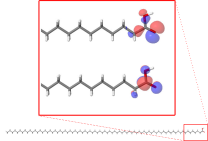
\includegraphics[scale=0.6]{Pics/NTOACID}
\caption{An interesting caption}
\end{figure}


\begin{figure}
\centering
\begin{subfigure}{0.3\linewidth}
\centering
\includegraphics[scale=0.6]{Pics/CISDENSE}
\caption{}
\end{subfigure}
$\Longrightarrow$
\begin{subfigure}{0.6\linewidth}
\centering
\includegraphics[scale=0.6]{Pics/CIS}
\caption{}
\end{subfigure}
\caption{An inte capwd m}
\end{figure}




% PAO CCLR not good! Look at Gunnar review article perhaps

% First appearance of local EOM-CCSD 
% Cra2002 https://aip.scitation.org/doi/pdf/10.1063/1.1537718

% First appearance of local CCLR CC2 (no doubles wrapping) Kat2006 https://aip.scitation.org/doi/pdf/10.1063/1.2339021
% Flaw: Domains dtermined from CCS, bad if not correponding to good approximat. ALso fixed during davidson

% Kat2009 https://aip.scitation.org/doi/pdf/10.1063/1.3237134
% FIxes Problem by refreshing domains

% state-specific PNOs from CIS(D) Hel2011 https://aip.scitation.org/doi/10.1063/1.3664902

% Hel2013 PNO-CC2 https://aip.scitation.org/doi/10.1063/1.4819071

% Hel2014 PNO-ADC2 https://www.sciencedirect.com/science/article/pii/S2210271X14001194?via%3Dihub

\section{Critical Stance on AO vs LMO} 

Distance criteria, or Mulliken/Löwdin pouplation
AO only for closed expressions (not for CCSD++) 
LOcal: ij cirteria, ij->ab criteria % https://www.sciencedirect.com/science/article/pii/S1574140006020044?via%3Dihub

\subsection{CC2}


\subsection{ADC}